\section{AWS Cloud Networking}
The following chapters describe several different technologies provided by amazon web services.

\begin{figure}[h]
    \centering
    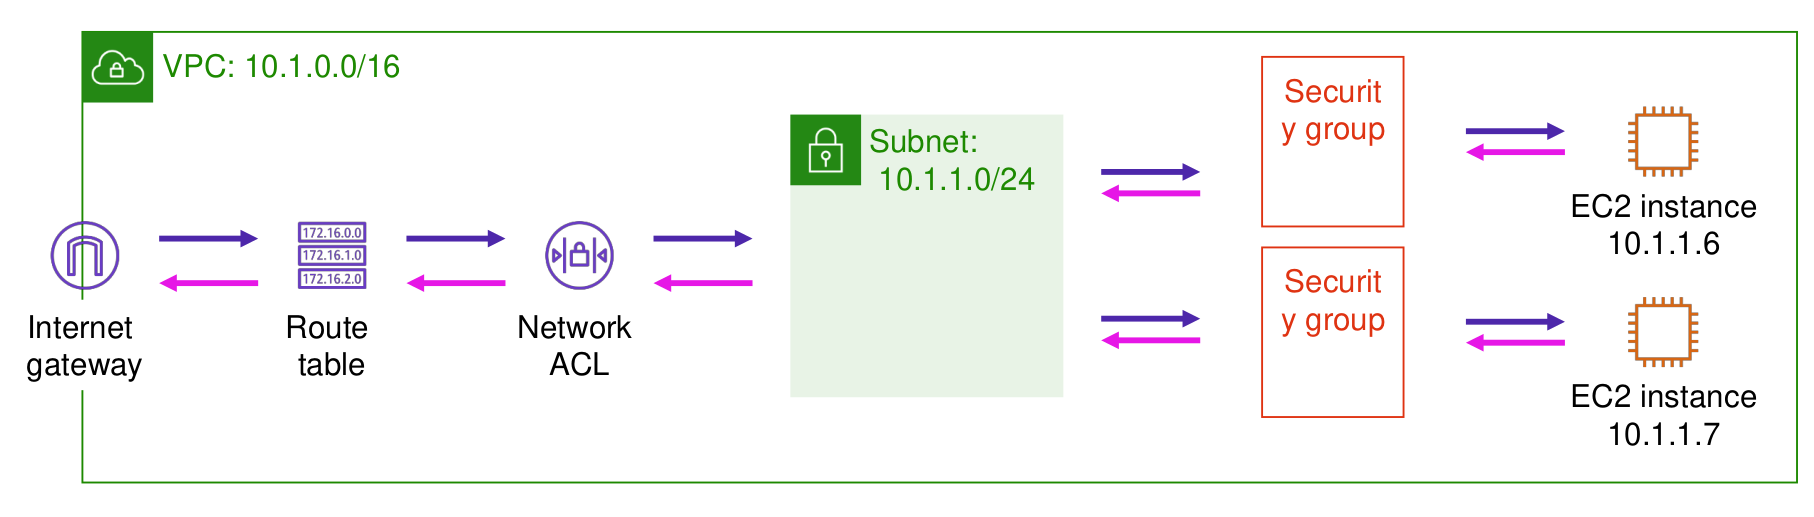
\includegraphics[width=\textwidth]{aws-multi-layer-architecture.png}
    \caption{AWS Layered Security Example}
\end{figure}

\subsection{Amazon VPC -- Virtual Private Cloud}
Isolated network for single workload. Placed in a single region, can span multiple availability zones (Amazon datacenters).

Contains private and public subnets for unique routing requirements. Don't overlap address space with internal networks!

Most use cases deploy multiple VPCs. Single VPC deployment can be suitable for:
\begin{itemize}
    \item Small, single applications managed by a small team
    \item High Performance Computing
    \item Identity Management
\end{itemize}

Limit: A maximum of 5 VPCs per region per account. Multi-Account setup used for large organizations with multiple IT teams.

\subsection{Internet Gateway}

Used to connect public instance IP addresses to the internet. 
Highly available and horizontally scaleable. 

Acts as default gateway for a public subnet route table.

\subsection{Route Table}
Every subnet must be associated with a route table. There is a default route table for every VPC.

\emph{Best practice}: use a custom route table fo reach subnet.

\subsection{Elastic IP Adress}
Static, public IPv4 addresses. Associated to an AWS account.

Can be associated with an instance or an elastic network interface. Remapping to other instances is possible. 
Useful for redundancy when load balancers are not an option.

\subsection{NAT Gateway}
Allows IP addresses from private subnets to access the internet or other AWS services. 
Outbound connections are possible, but not direct inbound connections.

Acts as default gateway for private route table.

\subsection{Security Groups}
A security group can be described as a stateful firewall that controls inbound and outbound traffic to AWS resources.
They act at the level of the instance or network interface.

\emph{Default config}: Block all inbound traffic, allow all outbound traffic. 

Custom security groups define Type, Protocol, Port Range, Source and Destination.

Chaining security groups allows to create a tiered architecture.

\subsection{Network ACLs}
Network access control lists act at the subnet level. 
They are stateless firewalls that require explicit rules for inbound and outbound traffic.

Custom Network ACLs are recommended for specific network security requirements only.

\subsection{Bastion Host}
Describes a host which is accessible from the internet to some specific users or public IPs.
Once connected to this host, access ot the internal network is allowed. 

This way, the internal host or instance only has to be accessible from one specific host.  